\chapter{Analysis and results}
\label{chap:analysis}

In the previous Chapter we have built a reinforcement learning environment with the use of the components which were described earlier in Chapter \ref{chap:preliminaries}.
The environment allows to simulate order placement on a historical order book that was described in Chapter \ref{chap:data}.
Furthermore, two agents were introduced, a Q-Learner which learns on private variables and a Deep Q-Network which learns on market variables.
The aim of this chapter is to run simulations and observe whether or not reinforcement learning is indeed capable of optimizing the placement of limit orders.
Throughout this chapter we make use of real world order books as well artificially created order books, whereas the latter allow to define distinctive price trends and eliminate the noise present in real market data.
We first analyze and discuss the effect of limit order placement in our given historical market by placing orders on each level.
This will provide knowledge of how well we should expect the reinforcement learners to perform.
Subsequently we make an attempt to build a strategy based on the private variables \textit{inventory} and \textit{time horizon} with the Q-Learner.
This serves as a benchmark for a naive reinforcement learner applied to the order placement problem, as well as the following simulations proceeded in which we consider market variables in the form of raw order book states and trades.
While applying market variables to the DQN agent we make use of both features, price and size of historical order as well as the price and size of historical trades, separately.
In doing this, we determine the capabilities and limitations not only by evaluating the received rewards but also by looking at the submitted actions of the agent.

\section{Order placement behaviour}

This section serves to investigate the relationship between the limit order placement and the received reward, for the corresponding orders.
The reward is denoted by the difference between the market price prior the order placement and the volume weighted average price (VWAP) paid, respectively received, as stated in Eq. \ref{setup:reward}.
The demonstrated methods are based on the related work described in Section \ref{sec:related-execution-behaviour} and provide understanding of the behaviour of order placement within a historical USD/BTC market and set a baseline for the reinforcement learners to come.
Particularly, the task is to buy or sell 1.0 BTC within a time horizon of 100 seconds, and evaluate achieved returns.
We recapitulate that according to \cite{nevmyvaka2005electronic, yingsaeree2012algorithmic} there are three obvious trading strategies in order to determine the execution price of an order (considering limit and market order types only):
\begin{enumerate}
    \item Submit a market order tor the entire amount immediately.
    \item Wait until the end of the time period and then go to the market with the entire amount.
    \item Submit a limit order at the beginning of the time period; then submitting a market order for the remainder of shares (if any) at the end of the interval.
\end{enumerate}
Having a total time horizon of 100 seconds available, the last approach is of interested in this analysis.
However, we investigate the behaviour on progressive increasing time horizons of starting from 10 seconds up to 100 seconds, as this demonstrates the discrete time steps to be taken by a learner.

\begin{figure}[H]
    \centering
    \makebox[\linewidth]{
        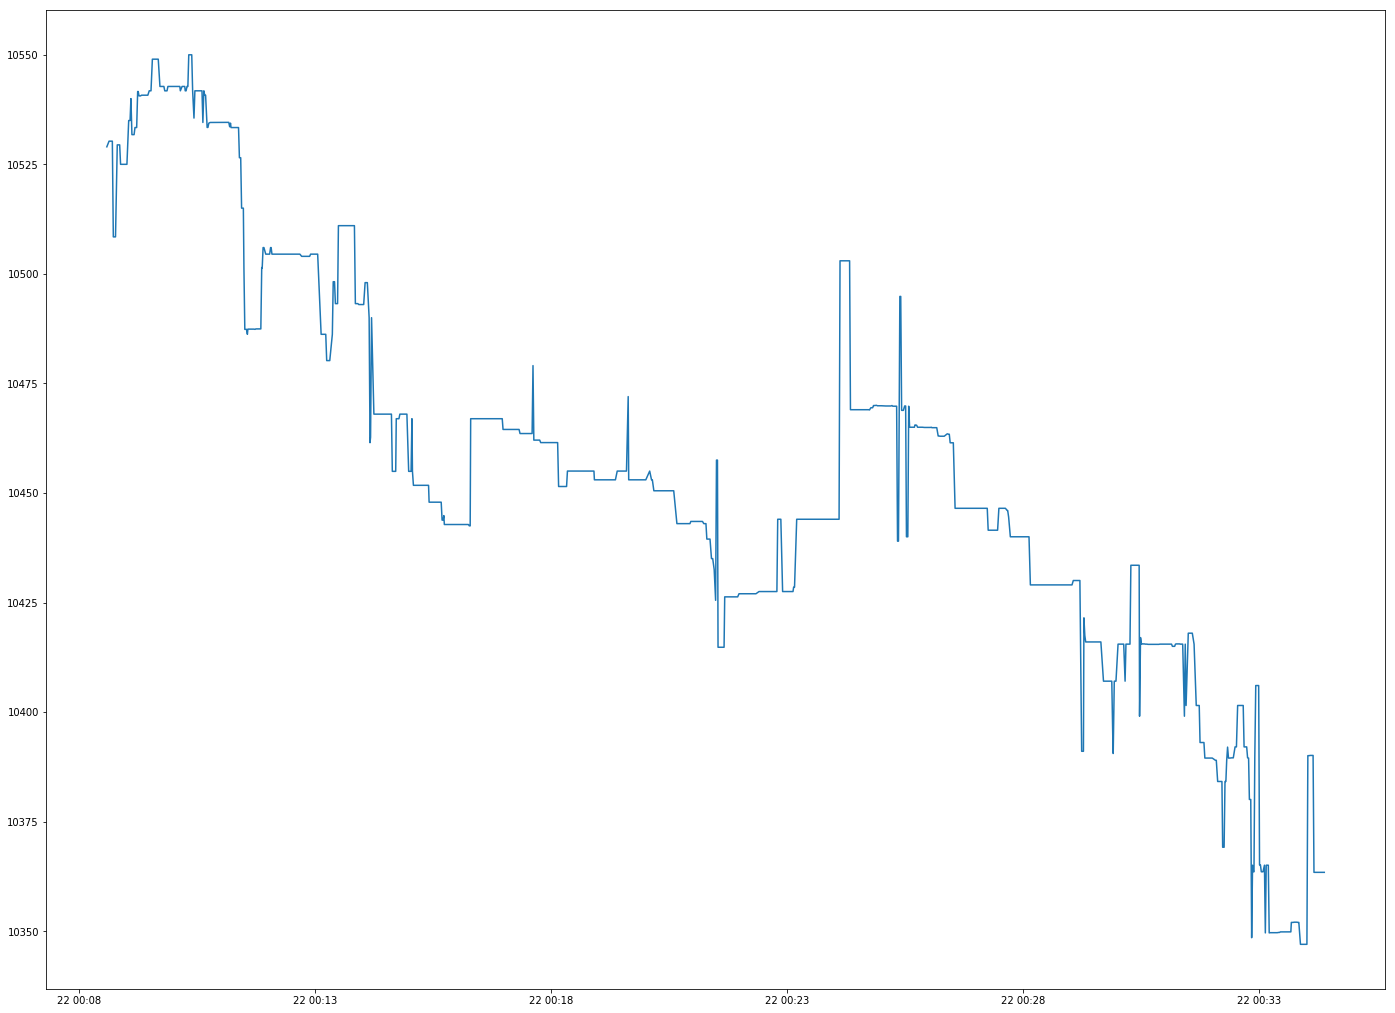
\includegraphics[width=10cm]{behaviour-price}
    }
    \caption{Bid/ask mid-price of a 30 minute recording of an order book.}
    \label{fig:behaviour-price}
\end{figure}
We have consciously chosen a sample order book which holds a 30 minute downwards trend, as indicated by the bid/ask mid-price in Figure \ref{fig:behaviour-price}, in order to have prior expectations about the effect of market and limit orders.
The expected return is being observed by the results of placing (e.g. cross-validating) 100 orders of size 1.0 BTC for a range of 201 limit levels ($-100...100$) with step size \$0.10 at a random point in the given data set.
\\
\\
\begin{figure}[H]
    \centering
    \begin{subfigure}[b]{0.45\textwidth}
        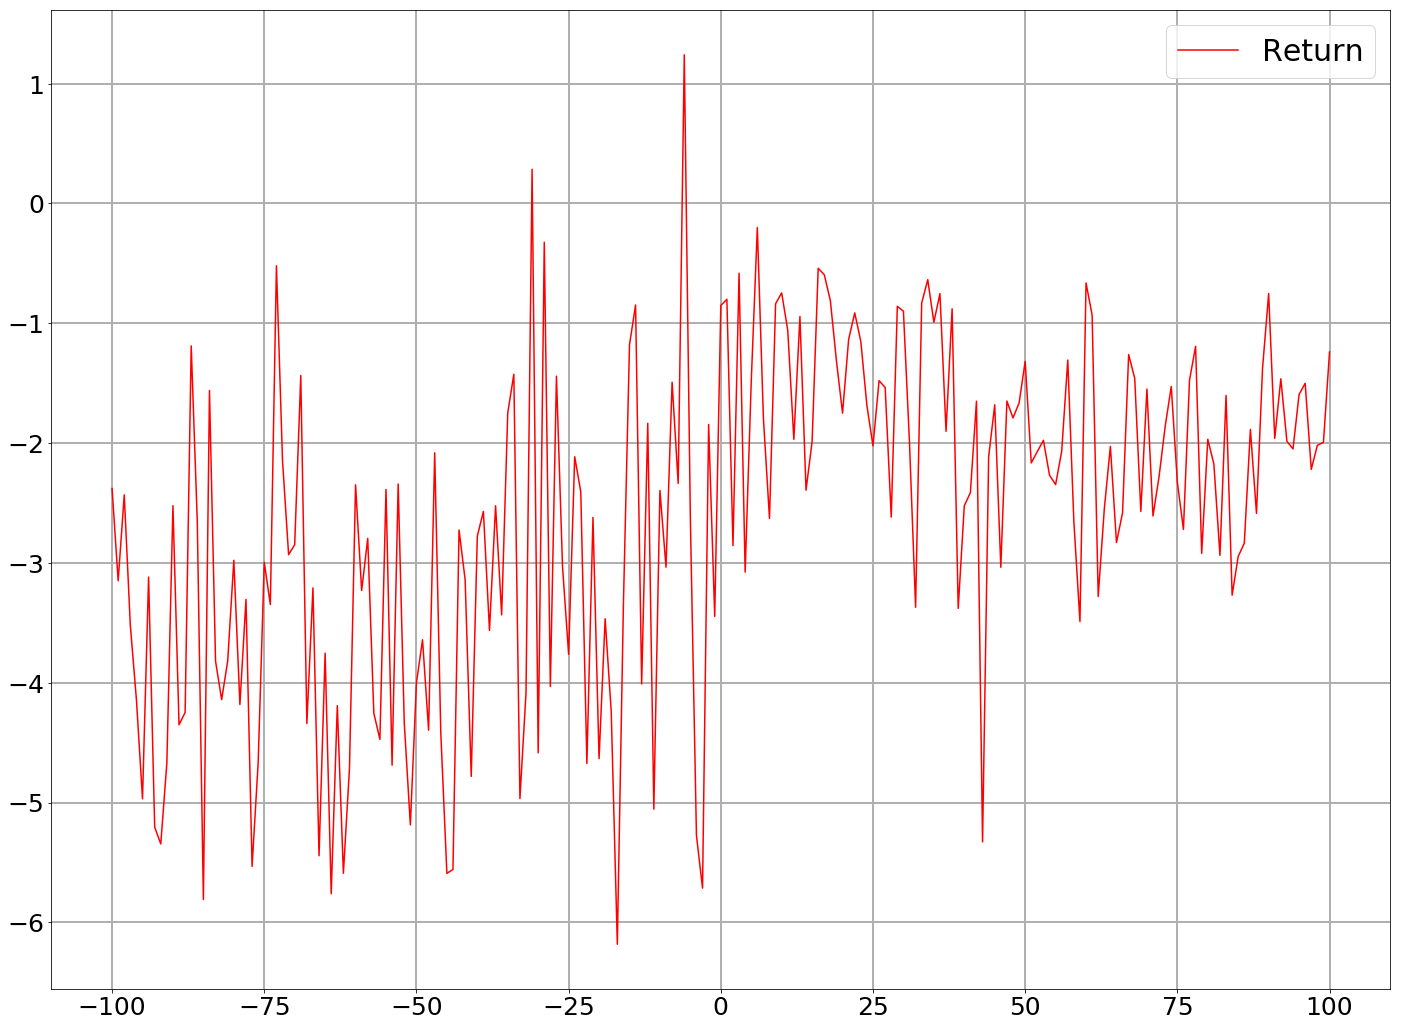
\includegraphics[width=\textwidth]{images/behaviour-10s-buy.png}
        \caption{Returns of buy orders}
        \label{fig:behvaiour-10s-buy}
    \end{subfigure}
    \begin{subfigure}[b]{0.45\textwidth}
        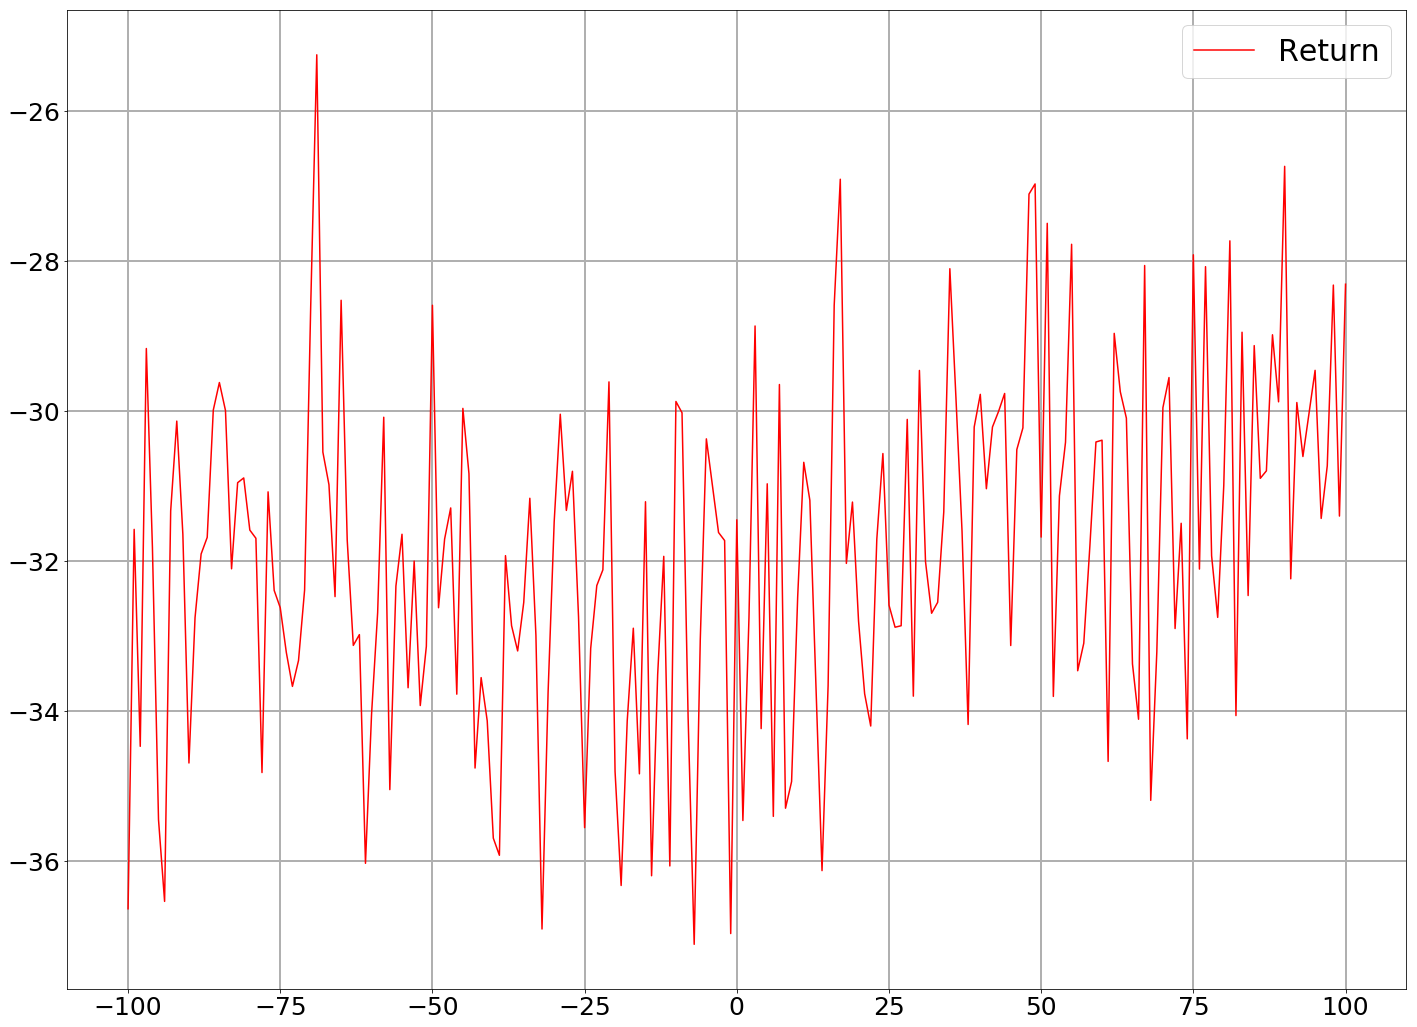
\includegraphics[width=\textwidth]{images/behaviour-10s-sell.png}
        \caption{Returns of sell orders}
        \label{fig:behvaiour-10s-sell}
    \end{subfigure}
    \caption{Return of orders executed within 10 seconds}
\end{figure}

\begin{figure}[H]
    \centering
    \begin{subfigure}[b]{0.45\textwidth}
        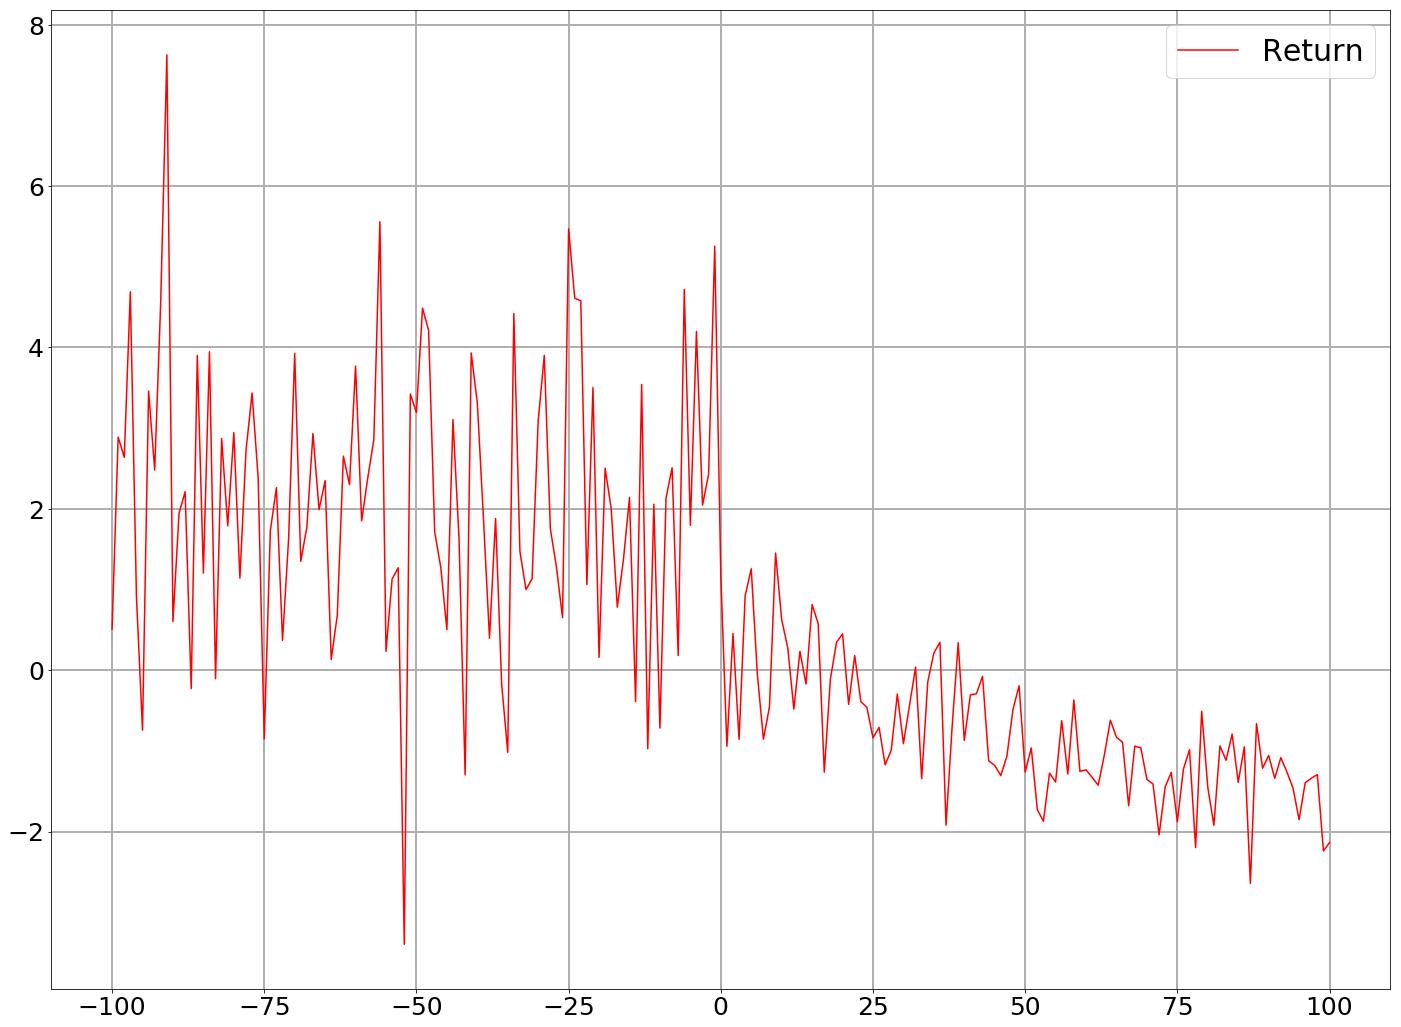
\includegraphics[width=\textwidth]{images/behaviour-30s-buy.png}
        \caption{Returns of buy orders}
        \label{fig:behvaiour-30s-buy}
    \end{subfigure}
    \begin{subfigure}[b]{0.45\textwidth}
        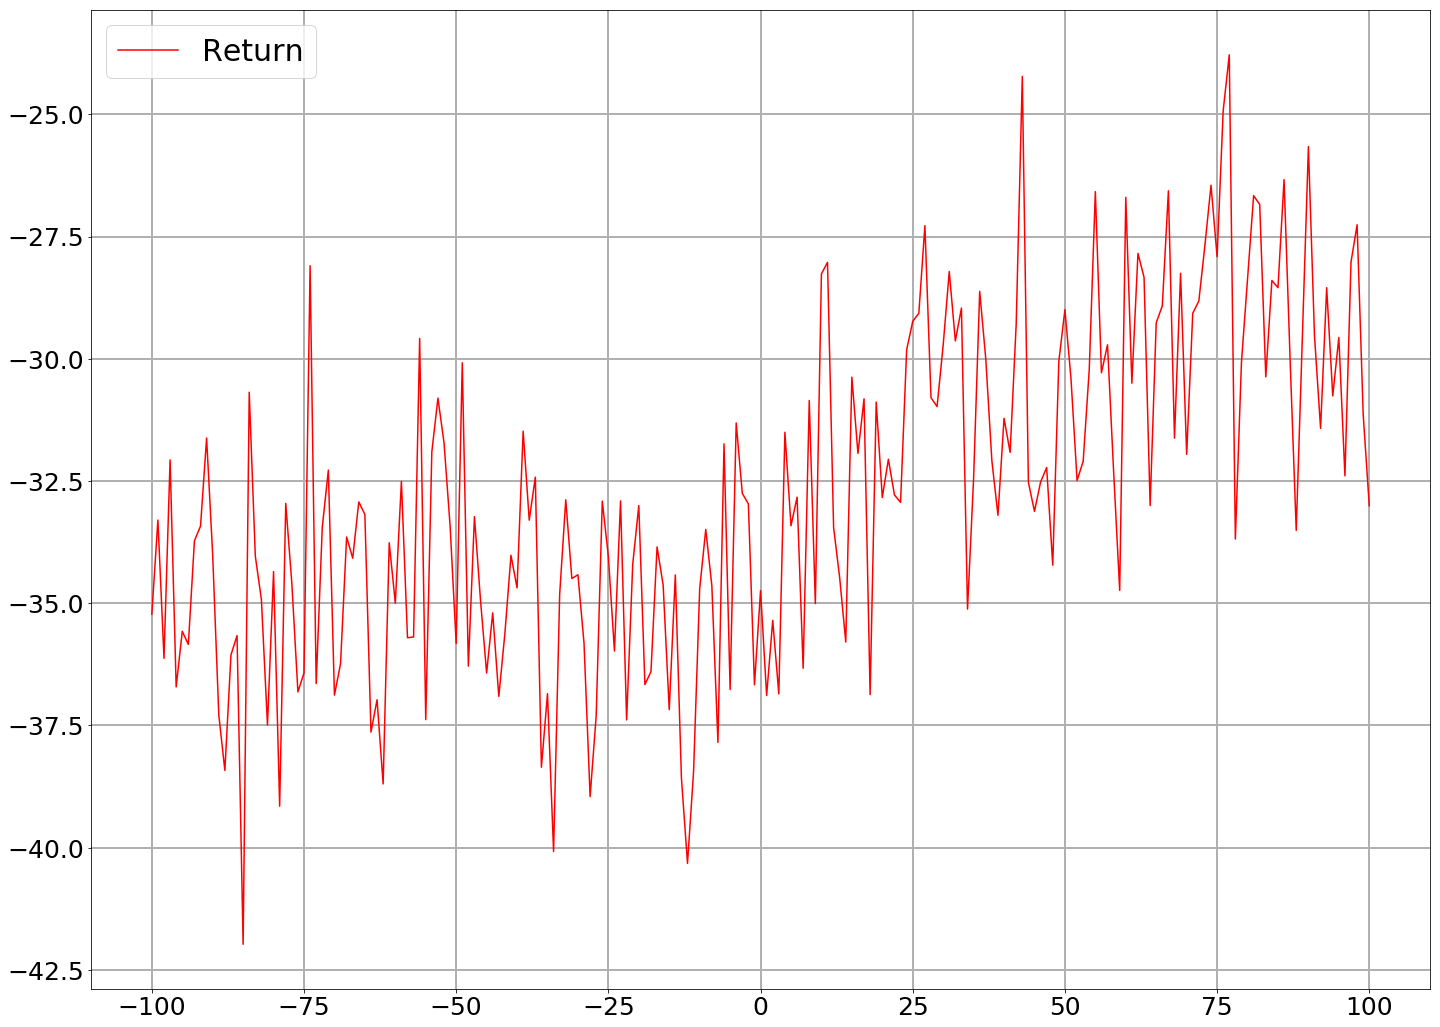
\includegraphics[width=\textwidth]{images/behaviour-30s-sell.png}
        \caption{Returns of sell orders}
        \label{fig:behvaiour-30s-sell}
    \end{subfigure}
    \caption{Return of orders executed within 30 seconds}
\end{figure}

\begin{figure}[H]
    \centering
    \begin{subfigure}[b]{0.45\textwidth}
        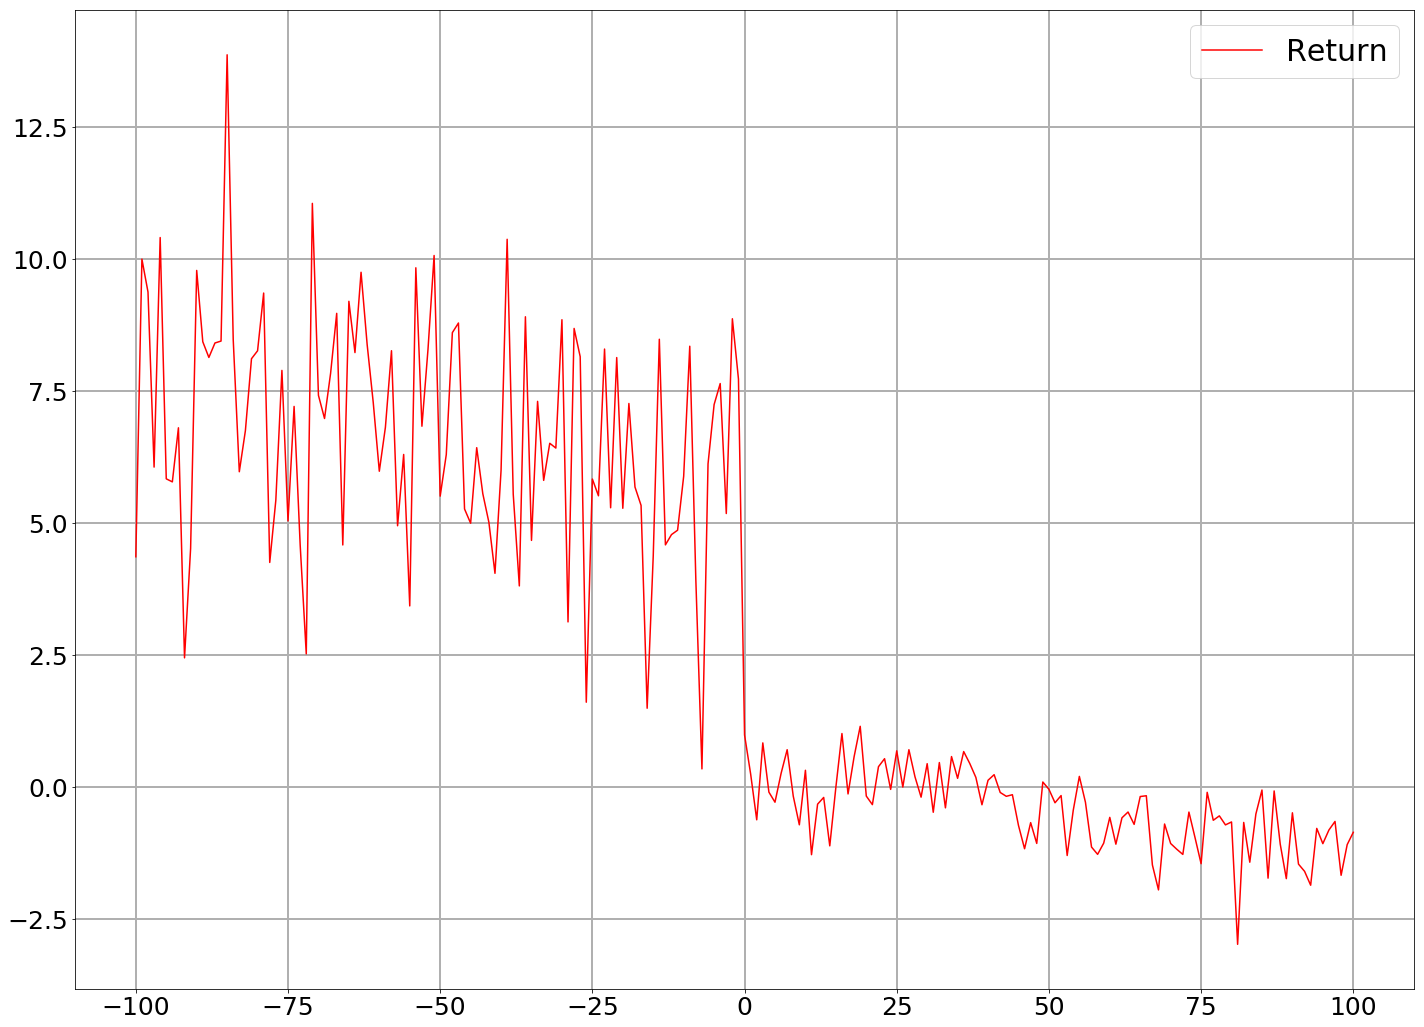
\includegraphics[width=\textwidth]{images/behaviour-60s-buy.png}
        \caption{Returns of buy orders}
        \label{fig:behvaiour-60s-buy}
    \end{subfigure}
    \begin{subfigure}[b]{0.45\textwidth}
        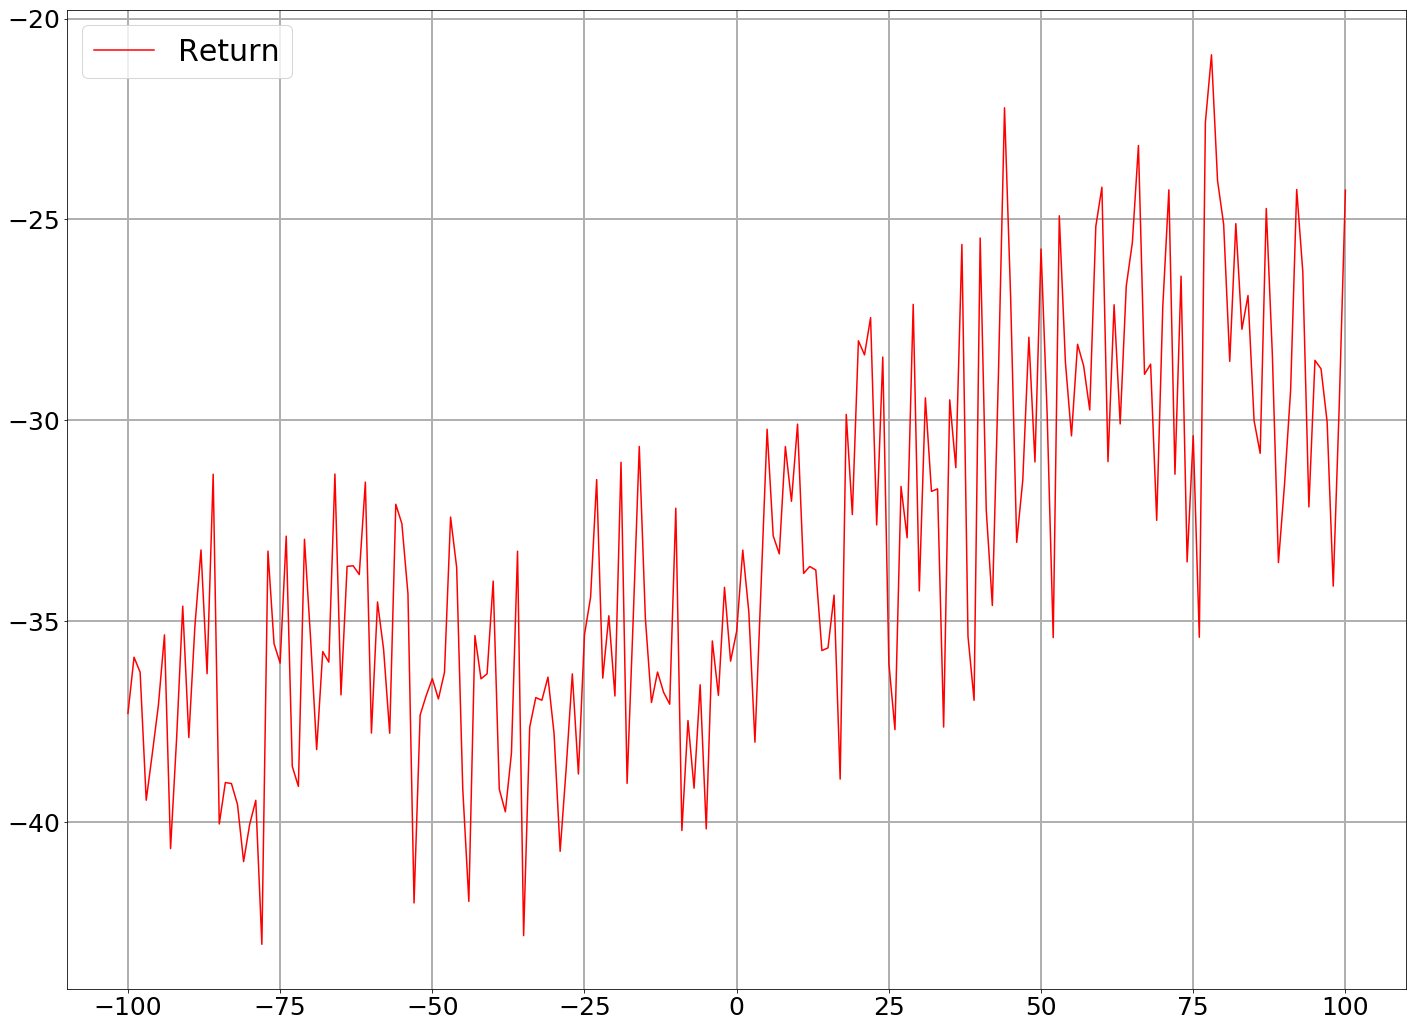
\includegraphics[width=\textwidth]{images/behaviour-60s-sell.png}
        \caption{Returns of sell orders}
        \label{fig:behvaiour-60s-sell}
    \end{subfigure}
    \caption{Return of orders executed within 60 seconds}
\end{figure}

\begin{figure}[H]
    \centering
    \begin{subfigure}[b]{0.45\textwidth}
        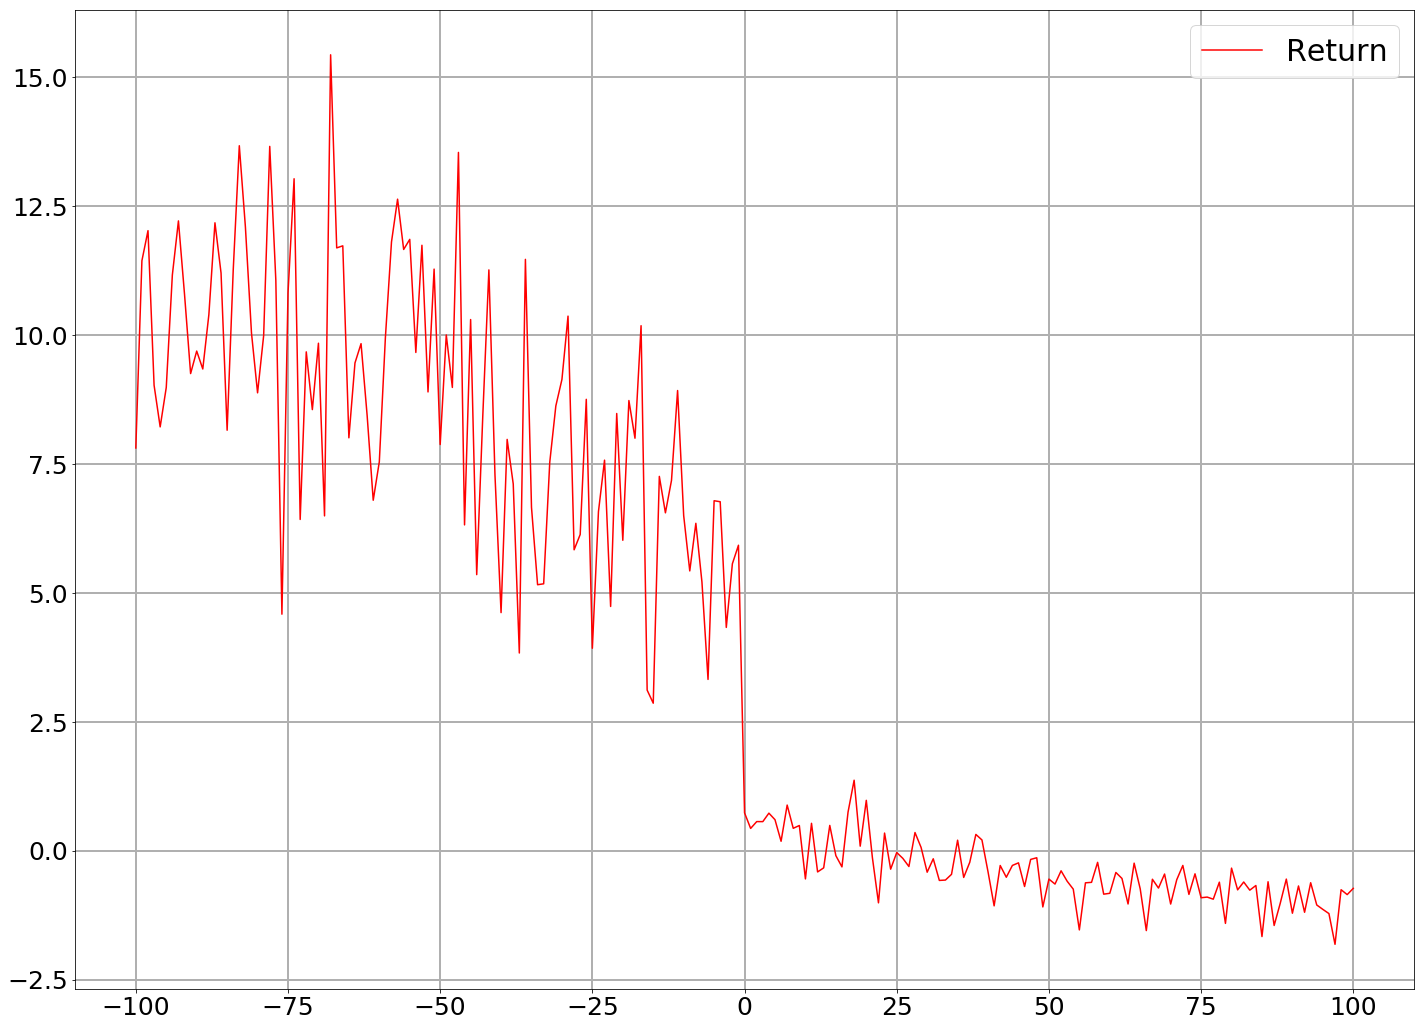
\includegraphics[width=\textwidth]{images/behaviour-100s-buy.png}
        \caption{Returns of buy orders}
        \label{fig:behvaiour-100s-buy}
    \end{subfigure}
    \begin{subfigure}[b]{0.45\textwidth}
        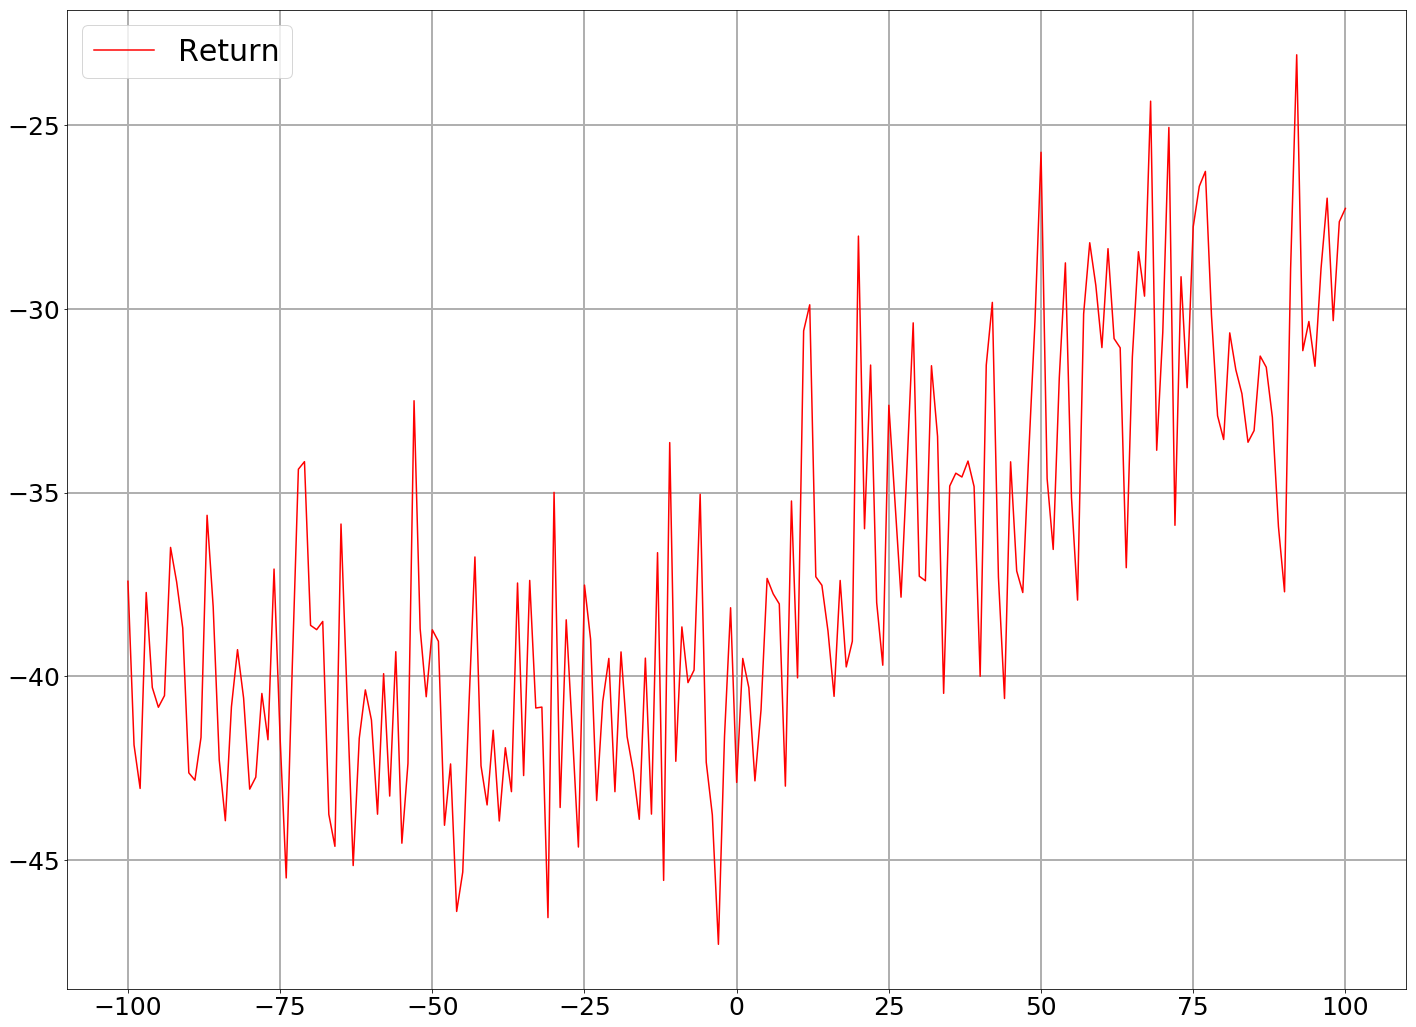
\includegraphics[width=\textwidth]{images/behaviour-100s-sell.png}
        \caption{Returns of sell orders}
        \label{fig:behvaiour-100s-sell}
    \end{subfigure}
    \caption{Return of orders executed within 100 seconds}
\end{figure}

\section{Q-Learning without market variables}

\section{Deep Q-Network on execution}

\section{Deep Q-Network on market making}

\section{Deep Q-Network with event flow data}
